\documentclass[twoside]{article}
%\usepackage{aistats2022}
% If your paper is accepted, change the options for the package
% aistats2022 as follows:
%
\usepackage[accepted]{aistats2022}
\usepackage{algorithm}
\usepackage{algpseudocode}
\usepackage{xcolor}
%
% This option will print headings for the title of your paper and
% headings for the authors names, plus a copyright note at the end of
% the first column of the first page.

% If you set papersize explicitly, activate the following three lines:
\special{papersize = 8.5in, 11in}
\setlength{\pdfpageheight}{11in}
\setlength{\pdfpagewidth}{8.5in}
\usepackage{mathtools}
\usepackage{amssymb}
\usepackage{xifthen}
\usepackage{bm}
\newcommand{\data}[0]{\mathcal{D}}
\newcommand{\vtheta}[0]{\boldsymbol \theta}
\newcommand{\Qfamily}[0]{\mathcal{Q}}
\newcommand{\KL}[2]{D_{KL}\left( #1 \Vert #2 \right)}
\newcommand{\E}[2]{\mathbb{E}_{#1} \left[ #2 \right]}
\newcommand{\R}[0]{\mathbb{R}}
\newcommand{\X}[0]{\mathcal{X}}
\newcommand{\A}[0]{\mathcal{A}}
\newcommand{\T}[0]{\mathcal{T}}

\newcommand{\eqdist}[0]{\,{\buildrel D \over =}\,}

\newcommand{\rvw}[0]{\mathbf{w}}
\newcommand{\rvu}[0]{\mathbf{u}}
\newcommand{\rvx}[0]{\textbf{x}}
\newcommand{\rvz}[0]{\textbf{z}}

\newcommand{\defeq}[0]{\vcentcolon=}
\newcommand{\eqdef}[0]{=\vcentcolon}
\newcommand{\distdefeq}[0]{\,\vcentcolon{\buildrel D \over =}\,}
\newcommand{\disteqdef}{\,{\buildrel D \over =}\vcentcolon\,}

\DeclareMathOperator*{\argmax}{arg\,max}
\DeclareMathOperator*{\argmin}{arg\,min}
% If you use natbib package, activate the following three lines:
\usepackage[round]{natbib}
\renewcommand{\bibname}{References}
\renewcommand{\bibsection}{\subsubsection*{\bibname}}

% If you use BibTeX in apalike style, activate the following line:
\bibliographystyle{apalike}

\begin{document}

\twocolumn[

  \aistatstitle{Normalizing Flows for Continous Distributional Reinforcement Learning}

  \aistatsauthor{ Ludvig Killingberg}

  \aistatsaddress{ Norwegian University of Science and Technology } ]

% \begin{abstract}
%   The Abstract paragraph should be indented 0.25 inch (1.5 picas) on
%   both left and right-hand margins. Use 10~point type, with a vertical
%   spacing of 11~points. The \textbf{Abstract} heading must be centered,
%   bold, and in point size 12. Two line spaces precede the
%   Abstract. The Abstract must be limited to one paragraph.
% \end{abstract}

\begin{abstract}
  % The Abstract paragraph should be indented 0.25 inch (1.5 picas) on
  % both left and right-hand margins. Use 10~point type, with a vertical
  % spacing of 11~points. The \textbf{Abstract} heading must be centered,
  % bold, and in point size 12. Two line spaces precede the
  % Abstract. The Abstract must be limited to one paragraph.
\end{abstract}

\section{Introduction}

% The submission versions of the papers are limited to 8 pages,
% plus any additional pages needed for references (and, optionally, supplementary
% material; see more details below). The camera-ready versions of the accepted
% papers are limited to 9 pages plus references and supplement.

% Papers are in 2 columns with the overall line width of 6.75~inches (41~picas).
% Each column is 3.25~inches wide (19.5~picas).  The space
% between the columns is .25~inches wide (1.5~picas).  The left margin is 0.88~inches (5.28~picas).
% Use 10~point type with a vertical spacing of
% 11~points. The font type must be Computer Modern.
% Please use US Letter size paper and not A4.

% Paper title is 16~point, caps/lc, bold, centered between 2~horizontal rules.
% Top rule is 4~points thick and bottom rule is 1~point thick.
% Allow 1/4~inch space above and below title to rules.

% Author descriptions are center-justified, initial caps.  The lead
% author is to be listed first (left-most), and the Co-authors are set
% to follow.  If up to three authors, use a single row of author
% descriptions, each one center-justified, and all set side by side;
% with more authors or unusually long names or institutions, use more
% rows.

% Use one-half line space between paragraphs, with no indent.

As an agent interacts with an environment, the environment and the agent's
policy interjects randomness into the return. Q-learning algorithms aim to
capture the mean of the (discounted) cumulative reward from interracting
with the environment. Distributional reinforcement learning (RL) in contrast
considers the randomness in the reward and aims to capture the following random
variable. In contrast to Q-learning algorithms, distributional reinforcement
learning algorithms aim to model distribution of the discounted cumulative
reward.

The difference in distributional reinforcement learning algorithms is mainly in
how the distribution is modeled.

\section{Background}

We consider the standard RL setting, where interaction between agent and
environment is modelled as a Markov Decision Process
\((\X, \A, R, P, \gamma)\)~\citep{puterman94}, where \(\X\) and \(\A\) denote
the state and action space respectively, \(R\) denotes the state-action
dependent reward function, \(P(\cdot \vert x, a)\) denotes the transition
probabilities, and \(\gamma \in [0,1]\) is the discount factor. A policy
\(\pi(\cdot \vert x)\) maps states to distributions over actions.

For an agent following policy \(\pi\), the return \(Z^\pi\),
or \emph{value distribution}~\citep{bellmare17}, is the sum of
discounted rewards along the agents trajectory

\begin{equation}
  Z^\pi(x, a) \defeq \sum_{t=0}^\infty{\gamma^t R(x_t,a_t)}
\end{equation}

\noindent
starting in state \(x_0 = x\), with \(a_0 = a\), \(a_t \sim \pi(\cdot \vert
x_t)\), and \(x_t \sim P(\cdot \vert x_{t-1}, a_{t-1})\).
The objective in RL can be summarized as finding the optimal policy \(\pi^*\)
that maximizes the expected return \(Q^\pi(x, a) \defeq \E{P, R, \pi}{Z^\pi(x, a)}
\). The most common approach is to find the unique fixed point of the Bellman
optimality operator~\citep{bellman57}

\begin{equation}
  \T Q^*(x, a) \defeq \E{}{R(x, a)} + \gamma \E{P}{\max_{a^\prime \in \A}
    Q^*(x^\prime, a^\prime)}.
\end{equation}

To approximate \(Q^*\), now usually modeled with a neural network \(Q_\theta\),
Q-learning~\citep{watkins89} iteratiely improves the estimate by minimizing the
squared temporal difference (TD) error

\begin{equation}
  \delta^2_t = \left[ r_t + \gamma \max_{a^\prime \in \A}
    Q_\theta(x_t, a^\prime) - Q_\theta(x_t, a_t) \right]^2
\end{equation}

for samples \((x_t, a_t, r_t, x_{t+1})\) in trajectory \(T\), observed as the
agent interracts with the environment according to an \(\epsilon\)-greedy policy
over \(Q_\theta\).

\subsection{Distributional Reinforcement Learning}

Rather than reducing the optimization problem to the expected return,
distributional reinforcement learning considers the full distribution of the
random variable \(Z^\pi\). Similar to the Bellman operator for the scalar
\(Q^\pi(x,a)\), we have a distributional Bellman operator

\begin{equation}
  \T Z^\pi(x, a) \distdefeq R(x, a) + \gamma Z^\pi(X^\prime, A^\prime)
\end{equation}

\noindent
where \(A \eqdist B\) denotes equality in distribution, i.e. random variable
\(A\) and \(B\) have the same distribution functions.

\subsubsection{Quantile Regression}

\subsection{Variational Inference}

% Third level headings are flush left, initial caps, bold, and in point
% size 10. Use one line space before the third level heading and one-half line
% space after the third level heading.

Lately, techniques for modelling complex distributions have have seen a surge
in popularity, particularily for generating realistic images. Given a dataset
\(\data\), we would like to find the distribution of parameters
\(p(\vtheta \vert \data)\). This is known as the posterior distribution. Using
full Bayesian inference we would calculate the posterior using Baye's theorem,
\begin{equation}
  p(\vtheta \vert \data) = \frac{p(\data \vert \vtheta)p(\vtheta)}{
    \int p(\data \vert \vtheta) p(\vtheta) d\vtheta}.
\end{equation}

Often, \(p\) is modelled by a neural network, which makes the denominator
intractable to compute. Variational inference provides an alternative to
computing the full posterior, by approximating \(p(\vtheta \vert \data)\) with
a distribution \(q(\vtheta)\) from a family of distributions \(\Qfamily\). We
do this by minimizing some measure of difference between the distributions. The
KL-divergence is a common choice since it has some useful properties we will
see later,
\begin{equation*}
  \KL{q(\vtheta)}{p(\vtheta \vert \data)} =
  \E{q(\vtheta)}{\log \frac{q(\vtheta)}{p(\vtheta \vert \data)}}.
\end{equation*}

Although the is not a metric (it is not symmetric, and does not obey the
triangle inequality), it is non-negative, and zero only when
\(q(\vtheta) = p(\vtheta \vert \data)\). Finding the approximation to the
posterior using the KL-divergence means solving the optimization problem,
\begin{equation*}
  q^* = \argmin_{q \in \Qfamily} \KL{q(\vtheta)}{p(\vtheta \vert \data)}.
\end{equation*}

Unfortunately, this is still a hard optimization problem. We can, however,
manipulate the KL-term to make the optimization problem tractable.
\begin{align*}
   & \KL{q(\vtheta)}{p(\vtheta \vert \data)} =
  \E{q(\vtheta)}{\log \frac{q(\vtheta)}{p(\vtheta \vert \data)}}                     \\
   & = \E{q(\vtheta)}{\log q(\vtheta)} - \E{q(\vtheta)}{\log p(\vtheta \vert \data)} \\
   & = \E{q(\vtheta)}{\log q(\vtheta)} - \E{q(\vtheta)}{\log
  \frac{p(\vtheta, \data)}{p(\data)}}                                                \\
   & = \E{q(\vtheta)}{\log q(\vtheta)} - \E{q(\vtheta)}{\log p(\vtheta, \data)} +
  \E{q(\vtheta)}{\log p(\data)}                                                      \\
   & = \E{q(\vtheta)}{\log q(\vtheta)} - \E{q(\vtheta)}{\log p(\vtheta, \data)} +
  \log p(\data)                                                                      \\
\end{align*}
This shows that minimizing the KL-divergence is the same as maximizing the
evidence lower bound (\textbf{ELBO}),
\begin{equation*}
  \mathrm{ELBO}(q; \vtheta, \data) = \E{q(\vtheta)}{\log p(\vtheta, \data)} -
  \E{q(\vtheta)}{\log q(\vtheta)}.
\end{equation*}

How close the approximate distribution, \(q(\vtheta))\), gets to the posterior
\(p(\vtheta \vert \data)\) depends on the family of distributions \(\Qfamily\).
We need to be able to quickly evaluate \(\E{q(\vtheta)}{p(\vtheta, \data)}\) and
\(\E{q(\vtheta)}{q(\vtheta}\), but we also want flexible, complex distributions,
such that \(q^* \in \Qfamily\) is close to \(p(\vtheta \vert \data)\). Most
early application of variational inference focused on mean-field for efficent
inference. Assuming factorization in the distributional family,
\begin{equation}
  \Qfamily =
  \left\{ q(\vtheta) \middle\vert \prod_{\theta_i \in \vtheta}{q(\theta_i)} \right\},
\end{equation}
is a strong restriction. It is unlikely that \(p(\vtheta \vert \data)\) will
factorize, and thus not be close to any \(q \in \Qfamily\). The nature of the
reverse KL-divergence will mean that the approximate posterior always
underestimates the variance of the true posterior.

\subsubsection{Normalizing Flows}
Normalizing flows is a method of transforming simple distributions into more
complex ones using parameterized functions. The change of variables formula is
used to construct a series of invertible transformations, where the probability
of the transformed variables can still be evaluated.

Let \(\rvZ\) be a random variable defined over the support \(S \subseteq \R^n\)
and a continous probability density function \(q(\rvz)\). Further, let \(v\) be
a continous, differentiable and invertible function from \(S\) to
\(T \in \R^n\), if we let \(\rvZ^\prime = v(\rvZ)\), then the probability
function \(q(\rvz^\prime)\) of \(\rvZ^\prime\) is given by
\begin{align}
  q(\rvz^\prime) & = q(\rvz) \left\lvert \det \left( \frac{\partial \rvz}{
  \partial \rvz^\prime} \right) \right\rvert \nonumber                                       \\
                 & = q(v^{-1}(\rvz^\prime)) \left\lvert \det \left( \frac{\partial}{\partial
    \rvz^\prime} v^{-1}(\rvz^\prime) \right) \right\rvert
  \label{eq:change_var_form1}
  % &= q(v^{-1}(\rvz^\prime)) \left\lvert \det \left( \frac{\partial}{\partial
  % \rvz} v(\rvz) \right) \right\rvert^{-1}
  % \label{eq:change_var_form2}
\end{align}

Normalizing flows takes advantage of this change of variables formula and create
a family of parameterized invertible transformation \(V\) with an easy to
compute jacobian. These transformations can be chained together to (usually)
create an arbitrarily complex transformation.
\begin{equation}
  \rvz_K = v_K \circ \dots \circ v_2 \circ v_1(\rvz_0),
\end{equation}
\begin{equation}
  \log q(\rvz_K) = \log q(\rvz_0) - \sum_{k=1}^K{\log \left\lvert \det
  \frac{\partial v_k}{\partial \rvz_k} \right\rvert}
\end{equation}

The \emph{planar flow} is a normalizing flow defined by a series of
transformations that expand and contract the distribution perpendicular to a
hyperplane \(\rvw^\top \rvz  + b\). For a smooth element-wise non-linear
function \(h(\cdot)\), with derivative \(h^\prime(\cdot)\), the planar flow is
defined as,

\begin{equation}
  v(\rvz) = \rvz + \rvu h(\rvw \rvz + b),
\end{equation}
\begin{equation}
  \det \left\lvert \frac{\partial v}{\partial \rvz} \right\rvert =
  \left\lvert 1 + \rvu^\top h^\prime(\rvw^\top \rvz + b) \rvw \right\rvert,
\end{equation}

\noindent
where \(\rvu\), \(\rvw\), and \(b\) are free parameters.
\(h(z) = \tanh(z)\) is a common choice. For this choice of non-linearity,
\(v\) is invertible if-and-only-if \(\rvw^\top u \geq -1\). To satisfy this
condition, \citet{rezende15} suggest starting with an arbitrary vector
\(\rvu\) and modify its component parallel to \(\rvw\), resulting in a new
vector \(\hat{\rvu}\) that satisfies \(\rvw^\top \hat{\rvu} \leq -1\).

\begin{equation*}
  m(x) = -1 + \log{(1 + e^x)}
\end{equation*}
\begin{equation}
  \hat{\rvu}(\rvu, \rvw) = \rvu + \left[m(\rvw^\top \rvu) -
    \rvw^\top \rvu \right] \frac{\rvw}{\lVert\rvw\rVert^2}
\end{equation}

\subsection{Conditional Normalizing Flows} \label{sec:cnf}
Although normalizing flows is a good method for approximating distributions,
they do not directly facilitate learning conditional likelihoods.
\citet{winkler19} propose learning conditional distributions with
\emph{conditional normalizing flows}. Given a conditioning variable
\(\rvx \in U\), a random variale \(\rvZ \in S \subseteq \R^n\), and a continous,
differentiable function \(v : S \times U \rightarrow T\), bijective in \(S\) and
\(T\), the probability function \(q(\rvz^\prime)\), where
\(\rvz^\prime = v(\rvz, \rvx)\), can be expressed as

\begin{align}
  q(\rvz^\prime \vert \rvx) & = q(\rvz \vert \rvx) \left\lvert \det
  \left( \frac{\partial \rvz}{\partial \rvz^\prime} \right) \right\rvert
  \nonumber                                                                                          \\
                            & = q(v^{-1}(\rvz^\prime, \rvx)) \left\lvert \det \left( \frac{\partial}
  {\partial \rvz^\prime} v^{-1}(\rvz^\prime, \rvx) \right) \right\rvert.
  \label{eq:cond_change_var_form1}
  % &= q(v^{-1}(\rvz^\prime; \rvx)) \left\lvert \det \left( \frac{\partial}
  % {\partial \rvz} v(\rvz; \rvx) \right) \right\rvert^{-1}
\end{align}

\noindent
Compared to Equation~\eqref{eq:change_var_form1}, all distributions are now
conditional, and the model has a conditional argument \(\rvx\).
\citet{winkler19} suggest three conditional modules:

\paragraph{Conditional Prior}
\begin{equation*}
  p(\rvz \vert \rvx) = \N(\rvz ; \mu(\rvx), \sigma^2(\rvx))
\end{equation*}
\paragraph{Conditional Split Prior}
\begin{equation*}
  p(\rvz_1 \vert \rvz_0, \rvx) =
  \N (\rvz ; \mu(\rvz_0, \rvx), \sigma^2(\rvz_0, \rvx))
\end{equation*}
\paragraph{Conditional Coupling}
\begin{equation*}
  \rvz^\prime_0 =
  s(\rvz_1, \rvx) \cdot \rvz_0 + t(\rvz_1, \rvx); \qquad \rvz^\prime_1 = \rvz_1
\end{equation*}

The functions \(\mu\), \(\sigma^2\), \(s\) and \(t\) are implemented using
neural networks.

\section{Our Algorithm}

We propose to use conditional normalizing flows to model the value distribution,
\(Z^\pi\), with a continous estimate. As opposed to previous work on
quantile regression methods, which aim to minimize the Wasserstein distance
to the target distribution, normalizing flows minimize the KL-divergence. Our
target is thus the KL-divergence from the value to the target distribution.

\begin{equation}
  \mathcal{L}_{\rvx,a}(\theta) \defeq \KL{Z_{\theta}(\rvx,a)}{\hat{\T}
    Z_{\tilde{\theta}}(\rvx,a)}
\end{equation}

Using conditional normalizing flows described in Section~\ref{sec:cnf}, we
define the value distribution model as a transformation of a
standard normal distribution conditioned on the state \(\rvx\).

% Similar to other DQN methods, we let \(Z_\theta(\rvx, a)\) be the \(a\)-th
% element of a function \(\tilde{Z}_\theta : \R^{\lvert \X \rvert}
% \rightarrow \R^{\lvert \A \rvert}\). This means that we need a conditional
% normalizing flow \(v_\theta : \R^{\lvert \X \rvert} \times \R^{\lvert \A \rvert}
% \rightarrow \R^{\lvert \A \rvert}\). Given that we have

Starting with a random variable \(S\) with a standard normal distribution
\(\N(0, I_{\lvert \A \rvert})\), we want a function \(v_\theta = v_{\theta_K}
\circ \dots \circ v_{\theta_2} \circ v_{\theta_1} \), such that
\(Z_\theta(\rvx, a) = v_\theta(S; \rvx^\prime)_a\). To learn \(v_\theta\) we note that
we can take the inverse transformation \(v^{-1}_\theta\) of the value
distribution to recover a random variable with the standard normal distribution,
i.e. \(S = v^{-1}_\theta(Z_\theta; \rvx)\). This further means that

\begin{equation}
  S^\prime \eqdist v^{-1}_\theta \left(\T v_\theta(S; \rvx^\prime); \rvx \right).
\end{equation}

Because the inverse transformation of the value distribution given its state is
standard normal, we can learn the parameters \(\theta\) using the
change-of-variables formula from Equation~\ref{eq:change_var_form1}.
Algorithm~\ref{alg:LTM} shows how to calculate the loss for this scheme.

\begin{algorithm}
  \caption{Flow-RL Loss}\label{alg:LTM}
  \textbf{Require:} \(N, v, v^{-1}, \theta, \tilde{\theta}\)\\
  \textbf{input} \(\rvx, a, r, \rvx^\prime, \gamma\)\\
  \hspace*{1em} {\color{gray} \# Take \(N\) samples from the value distribution.}\\
  \hspace*{1em} \textbf{for} \(i = 1 \dots N\)\\
  \hspace*{2em} \(\epsilon_i \sim \N \left(0, 1 \right)\)\\
  \hspace*{2em} \textbf{for} \(a^\prime \in \A\)\\
  \hspace*{3em} \(Z_{\tilde{\theta}}(\rvx^\prime, a^\prime)_i \gets v_{\tilde{\theta}}(\epsilon_i; \rvx^\prime)_{a^\prime}\)\\
  \hspace*{2em} \textbf{end}\\
  \hspace*{1em} \textbf{end}\\
  \\\hspace*{1em} {\color{gray} \# Compute greedy next action.}\\
  \hspace*{1em} \(a^* \gets \argmax_{a^\prime} \frac{1}{N} \sum_{i=1}^N Z_{\tilde{\theta}}(\rvx^\prime, a^\prime)_i\)\\
  \\\hspace*{1em} {\color{gray} \# Calculate loss terms for each sample.}\\
  \hspace*{1em} \textbf{for} \(i = 1 \dots N\)\\
  \hspace*{2em} {\color{gray} \# Apply the distributional Bellman operator.}\\
  \hspace*{2em} \(\hat{Z}_{\tilde{\theta}}(\rvx, a)_i \gets r + \gamma Z_{\tilde{\theta}}(\rvx^\prime, a^*)_i\)\\
  \hspace*{2em} {\color{gray} \# Calculate negative log-likelihood loss term.}\\
  \hspace*{2em} \(\delta_i \gets \frac{1}{2} v_{\theta}^{-1}
  \left(\hat{Z}_{\tilde{\theta}}(\rvx, a)_i; \rvx \right)^2\)\\
  \hspace*{2em} {\color{gray} \# Calculate log-derivative of \(v^{-1}_\theta\).}\\
  \hspace*{2em} \(\rho_i \gets \log \left\lvert \frac{\partial v_{\theta}^{-1} \left(\hat{Z}_{\tilde{\theta}}(\rvx, a)_i; \rvx \right)}{\hat{Z}_{\tilde{\theta}}(\rvx, a)_i} \right\rvert\)\\
  \hspace*{1em} \textbf{end}\\
  \textbf{output} \(\frac{1}{N}\sum_{i=1}^N \delta_i - \rho_i\)
\end{algorithm}

% \begin{equation}
%   \T \tilde{Z}_\theta(\rvx)_a \defeq R(\rvx, a) + \max_{a^\prime \in \A}
%   \tilde{Z}_\theta(\rvx^\prime)_{a^\prime}
% \end{equation}

% \noindent
% we can see that any learning signal would only come for a single action. This
% means that we need an elementwise flow so that we can learn each dimension
% independently. Given elementwise conditional normalizing flow \(v_\theta\), we
% define the loss function as

% \begin{multline}
%   \mathcal{L}_{\rvx, a}(\theta) \defeq \log p(v_\theta^{-1} (\rvx, v_{\tilde{
%   \theta}} (\rvx^\prime, \vepsilon))_a; 0, 1) \\- \log
%   \left\lvert \frac{\partial v^{-1}_{\theta}(\rvx, v_{\tilde{
%   \theta}} (\rvx^\prime, \vepsilon))_a}{\partial v_{\tilde{
%   \theta}} (\rvx^\prime, \vepsilon)_a} \right\rvert; \quad
%   \vepsilon \sim \N(0, I_{\lvert \A \rvert})
% \end{multline}

The most popular normalizing flows right now are buildt for large dimensional
spaces such as images. This includes coupling and autoregressive flows. Planar
flow is very easy to turn elementwise, but unfortunately does not have a closed
form inverse for most functions of \(h\). Although it does have one for
piecewise linear funcitons, those do not have second derivative, hence the
gradient of the log absolute determinant would be zero. This would mean it can
not learn appropriate transformations. Instead we define our own flow.

Equation~\ref{eq:luddeflow} shows the definitiona of the forward transformation
\(v(\cdot; b, c, d)\), with 3 free parameters \(b, c, d\). Unlike the planar
flow, this function has a closed form inverse and is differentiable given any values for these
parameters, hence no reparameterization is necessary. Equation~\ref{eq:luddeflow_inv} and
Equation~\ref{eq:luddeflow_grad} show the closed form inverse and gradient respectively.

\begin{equation}
  v(z; b, c, d) = \sign(z - c) \log \left( e^{\lvert x - c \rvert}
  + e^{b} - 1 \right) + d \label{eq:luddeflow}
\end{equation}

\begin{equation}
  \frac{\partial v(z; b, c, d)}{\partial z} = \frac{e^{\lvert x - c \rvert}}
  {e^{\lvert x - c \rvert} + e^{b} - 1}
  \label{eq:luddeflow_grad}
\end{equation}

\begin{equation}
  v^{-1}(z^\prime; b, c, d) = v(z^\prime; -b, d, c) \label{eq:luddeflow_inv}
\end{equation}

Figure~\ref{fig:luddeflow} shows the effect of the free parameters. A simple
description is that \(b\) changes the
\emph{linearity} of the function (\(v\) is linear when \(b = 0\), an expansive
mapping when \(b < 0\) and a contraction when \(b > 0\)), \(c\) shifts \(v\) horizontally, and \(d\) shifts \(v\) vertically.

\begin{figure}[ht]
  \vspace{.3in}
  % \centerline{\fbox{This figure intentionally left non-blank}}
  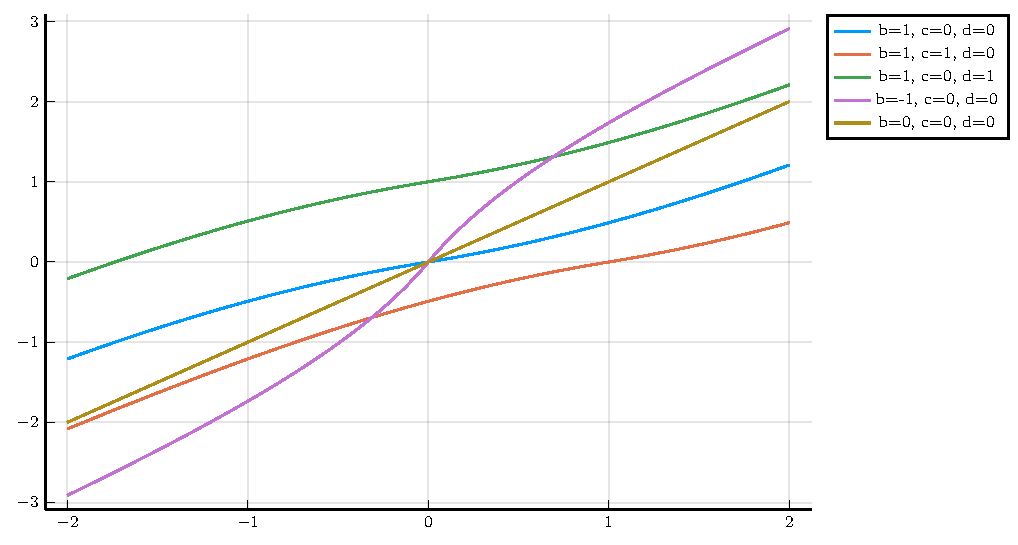
\includegraphics[width=\columnwidth]{new_flow.pdf}
  \vspace{.3in}
  \caption{Illustration of the effect the free parameters have on the function.
  }\label{fig:luddeflow}
\end{figure}

\begin{figure}[ht]
  \vspace{.3in}
  % \centerline{\fbox{This figure intentionally left non-blank}}
  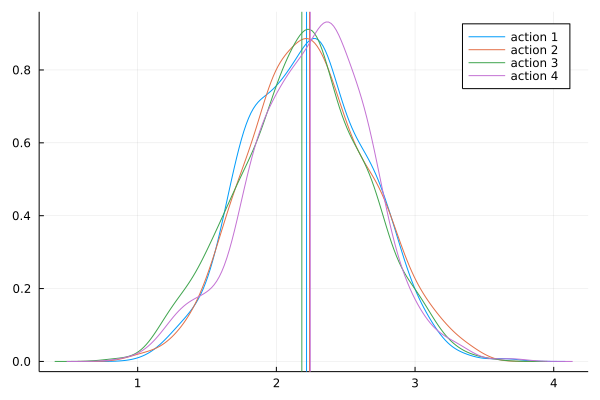
\includegraphics[width=\columnwidth]{qdistr_6100.png}
  \vspace{.3in}
  \caption{Learned \(Z^\pi\)-distribution during an episode in Breakout.}
\end{figure}

% \paragraph{Fourth Level Heading}

% Fourth level headings must be flush left, initial caps, bold, and
% Roman type.  Use one line space before the fourth level heading, and
% place the section text immediately after the heading with no line
% break, but an 11 point horizontal space.

%%%
% \subsection{Citations, Figure, References}


% \subsubsection{Citations in Text}

% Citations within the text should include the author's last name and
% year, e.g., (Cheesman, 1985). 
% %Apart from including the author's last name and year, citations can follow any style, as long as the style is consistent throughout the paper.  
% Be sure that the sentence reads
% correctly if the citation is deleted: e.g., instead of ``As described
% by (Cheesman, 1985), we first frobulate the widgets,'' write ``As
% described by Cheesman (1985), we first frobulate the widgets.''


% The references listed at the end of the paper can follow any style as long as it is used consistently.

%Be sure to avoid
%accidentally disclosing author identities through citations.

% \subsubsection{Footnotes}

% Indicate footnotes with a number\footnote{Sample of the first
%   footnote.} in the text. Use 8 point type for footnotes. Place the
% footnotes at the bottom of the column in which their markers appear,
% continuing to the next column if required. Precede the footnote
% section of a column with a 0.5 point horizontal rule 1~inch (6~picas)
% long.\footnote{Sample of the second footnote.}

% \subsubsection{Figures}

% All artwork must be centered, neat, clean, and legible.  All lines
% should be very dark for purposes of reproduction, and art work should
% not be hand-drawn.  Figures may appear at the top of a column, at the
% top of a page spanning multiple columns, inline within a column, or
% with text wrapped around them, but the figure number and caption
% always appear immediately below the figure.  Leave 2 line spaces
% between the figure and the caption. The figure caption is initial caps
% and each figure should be numbered consecutively.

% Make sure that the figure caption does not get separated from the
% figure. Leave extra white space at the bottom of the page rather than
% splitting the figure and figure caption.
% \begin{figure}[ht]
% \vspace{.3in}
% \centerline{\fbox{This figure intentionally left non-blank}}
% \vspace{.3in}
% \caption{Sample Figure Caption}
% \end{figure}

% \subsubsection{Tables}

% All tables must be centered, neat, clean, and legible. Do not use hand-drawn tables.
% Table number and title always appear above the table.
% See Table~\ref{table}.

% Use one line space before the table title, one line space after the table title,
% and one line space after the table. The table title must be
% initial caps and each table numbered consecutively.

% \begin{table}[ht]
% \caption{Sample Table Title} \label{table}
% \begin{center}
% \begin{tabular}{ll}
% \textbf{PART}  &\textbf{DESCRIPTION} \\
% \hline \\
% Dendrite         &Input terminal \\
% Axon             &Output terminal \\
% Soma             &Cell body (contains cell nucleus) \\
% \end{tabular}
% \end{center}
% \end{table}

% \section{SUPPLEMENTARY MATERIAL}

% If you need to include additional appendices during submission, you can include them in the supplementary material at the end of this file. It can be in either one- or two-column format.

% In addition, you can submit a single file of additional non-textual supplementary material, which should be a ZIP file containing, e.g., code. 
% Note that reviewers are under no obligation to examine your supplementary material. 

% \section{SUBMISSION INSTRUCTIONS}

% To submit your paper to AISTATS 2022, please follow these instructions.

% \begin{enumerate}
%     \item Download \texttt{aistats2022.sty}, \texttt{fancyhdr.sty}, and \texttt{sample\_paper.tex} provided in our starter pack. 
%     Please, do not modify the style files as this might result in a formatting violation.

%     \item Use \texttt{sample\_paper.tex} as a starting point.
%     \item Begin your document with
%     \begin{flushleft}
%     \texttt{\textbackslash documentclass[twoside]\{article\}}\\
%     \texttt{\textbackslash usepackage\{aistats2022\}}
%     \end{flushleft}
%     The \texttt{twoside} option for the class article allows the
%     package \texttt{fancyhdr.sty} to include headings for even and odd
%     numbered pages.
%     \item When you are ready to submit the manuscript, compile the latex file to obtain the pdf file.
%     \item Check that the content of your submission, \emph{excluding} references, is limited to \textbf{8 pages}. The number of pages containing references (and, optionally, supplementary material) is not limited. Note that the camera-ready version can have \textbf{9 pages}, see details below.
%     \item (Optional) Upload the ZIP file along with other supplementary material files to the CMT website.
% \end{enumerate}

% \subsection{Camera-ready Papers}

%For the camera-ready paper, if you are using \LaTeX, please make sure
%that you follow these instructions.  
% (If you are not using \LaTeX,
%please make sure to achieve the same effect using your chosen
%typesetting package.)

% If your papers are accepted, you will need to submit the camera-ready version. Please make sure that you follow these instructions:
% \begin{enumerate}
%     %\item Download \texttt{fancyhdr.sty} -- the
%     %\texttt{aistats2022.sty} file will make use of it.
%     \item Change the beginning of your document to
%     \begin{flushleft}
%     \texttt{\textbackslash documentclass[twoside]\{article\}}\\
%     \texttt{\textbackslash usepackage[accepted]\{aistats2022\}}
%     \end{flushleft}
%     The option \texttt{accepted} for the package
%     \texttt{aistats2022.sty} will write a copyright notice at the end of
%     the first column of the first page. This option will also print
%     headings for the paper.  For the \emph{even} pages, the title of
%     the paper will be used as heading and for \emph{odd} pages the
%     author names will be used as heading.  If the title of the paper
%     is too long or the number of authors is too large, the style will
%     print a warning message as heading. If this happens additional
%     commands can be used to place as headings shorter versions of the
%     title and the author names. This is explained in the next point.
%     \item  If you get warning messages as described above, then
%     immediately after $\texttt{\textbackslash
%     begin\{document\}}$, write
%     \begin{flushleft}
%     \texttt{\textbackslash runningtitle\{Provide here an alternative
%     shorter version of the title of your paper\}}\\
%     \texttt{\textbackslash runningauthor\{Provide here the surnames of
%     the authors of your paper, all separated by commas\}}
%     \end{flushleft}
%     Note that the text that appears as argument in \texttt{\textbackslash
%       runningtitle} will be printed as a heading in the \emph{even}
%     pages. The text that appears as argument in \texttt{\textbackslash
%       runningauthor} will be printed as a heading in the \emph{odd}
%     pages.  If even the author surnames do not fit, it is acceptable
%     to give a subset of author names followed by ``et al.''

%     %\item Use the file sample\_paper.tex as an example.

%     \item The camera-ready versions of the accepted papers are 9
%       pages, plus any additional pages needed for references (and,
%       optionally, supplementary material).

%     \item If you need to include additional appendices,
%       you can include them in the supplementary
%       material at the end of this file. There is no page limit
%       for the supplementary material.

%     \item Please, do not change the layout given by the above
%       instructions and by the style file.

% \end{enumerate}

% \subsubsection*{Acknowledgements}
% All acknowledgments go at the end of the paper, including thanks to reviewers who gave useful comments, to colleagues who contributed to the ideas, and to funding agencies and corporate sponsors that provided financial support. 
% To preserve the anonymity, please include acknowledgments \emph{only} in the camera-ready papers.


% \subsubsection*{References}

% References follow the acknowledgements.  Use an unnumbered third level
% heading for the references section.  Please use the same font
% size for references as for the body of the paper---remember that
% references do not count against your page length total.

\bibliography{references.bib}



% %%%%%%%%%%%%%%%%%%%%%%%%%%%%%%%%%%%
% %%%%%% SUPPLEMENT (OPTIONAL) %%%%%%
% %%%%%%%%%%%%%%%%%%%%%%%%%%%%%%%%%%%

% \clearpage
% \appendix

% \thispagestyle{empty}


% % For one-column format, uncomment the following:
% \onecolumn \makesupplementtitle
% % For two-column format, uncomment the following:
% %\twocolumn[ \makesupplementtitle ]

% \section{FORMATTING INSTRUCTIONS FOR THE SUPPLEMENTARY MATERIAL}

% Your supplementary material should go here. It may be in one-column or two-column format. To display the supplementary material in two-column format, comment out the line
% \begin{verbatim}
% \onecolumn \makesupplementtitle
% \end{verbatim}
% and uncomment the following line:
% \begin{verbatim}
% \twocolumn[ \makesupplementtitle ]
% \end{verbatim}

% Please submit your paper (including the supplementary material) as a single PDF file. Besides the PDF file, you may submit a single file of additional non-textual supplementary material, which should be a ZIP file containing, e.g., code.

% If you require to upload any video as part of the supplementary material of your camera-ready submission, do not submit it in the ZIP file. Instead, please send us via email the URL containing the video location.

% Note that reviewers are under no obligation to examine your supplementary material.

% \section{MISSING PROOFS}

% The supplementary materials may contain detailed proofs of the results that are missing in the main paper.

% \subsection{Proof of Lemma 3}

% \textit{In this section, we present the detailed proof of Lemma 3 and then [ ... ]}

% \section{ADDITIONAL EXPERIMENTS}

% If you have additional experimental results, you may include them in the supplementary materials.

% \subsection{The Effect of Regularization Parameter}

% \textit{Our algorithm depends on the regularization parameter $\lambda$. Here we illustrate the effect of this parameter on the performance of our algorithm [ ... ]}


\end{document}

